usadadas das formula

{\Large%-------->>FÓRMULA<<----------
\[
F = k \frac{{|Q|}}{{r^2}}
\]
}%----------
\textbf{Enumeración alfabética:} 
\begin{enumerate}[label=\alph*.]

  \item \textbf{Fuerza eléctrica}

  %\input{e1-fuerza-e}
  
  \item \textbf{Campo eléctrico}

  %\input{e1-campo-e}

\end{enumerate}

\textbf{Código:} 
\begin{minted}[
  breaklines=true,
  breaksymbolleft=\hspace{0pt},
  breaksymbolright={},
  mathescape,
  bgcolor=LightGray,
  linenos=false,
]{python}
# Note: $\pi=\lim_{n\to\infty}\frac{P_n}{d}$
title = "Hello World"

sum = 0
for i in range(10):
 sum += i

grid_layout = QGridLayout()  
        botones = [
            
        ]
        
        for btn_text, row, col, rowspan, colspan in [(b[0], b[1], b[2], 1, 1) if len(b) == 3 else b for b in botones]:
            button = QPushButton(btn_text)
            button.clicked.connect(self.on_click)
            if btn_text == 'Calcular':
                button.setStyleSheet("background-color: green; color: white;")
            else:
                button.setStyleSheet("background-color: white;")
            grid_layout.addWidget(button, row, col, rowspan, colspan)
        
        layout.addLayout(grid_layout)
        self.setLayout(layout)
    
def on_click(self):
        sender = self.sender()
        text = sender.text()
        
        if text == 'Borrar':
            current_text = self.funcion.text()
            if current_text:
                self.funcion.setText(current_text[:-1])
        elif text == 'Calcular':
            self.interpretar()
        else:
            self.funcion.setText(self.funcion.text() + text)


\end{minted}

\textbf{Código:} 
% Iniciar numeracio: linenos, firstnumber=10
\inputminted[
  breaklines=true,
  breaksymbolleft=\hspace{0pt},
  breaksymbolright={},
  mathescape,
  bgcolor=LightGray,
  linenos=false,
]
{python}{code/lineas_campo_grafica.py}


\textbf{Figura:} 
%--------------->>FIGURA<<------------------
\begin{figure}[H]
  \centering
  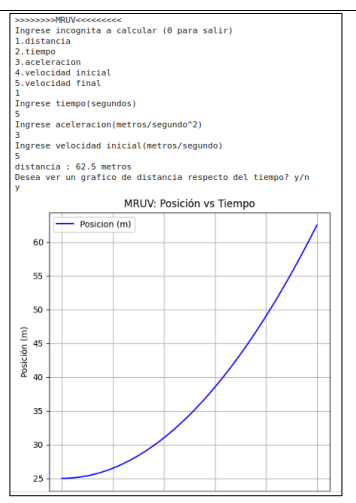
\includegraphics[width=0.65\linewidth]{img/ejecucion.png}
  \caption{\centering
    dasdasdasdadescripcion
  }
\end{figure}%-----





